\section{Design}
\label{s:gen}

This section describes \sys's design for constraint generation and
solving, as shown in \autoref{f:flow}.

\sys generates three categories of constraints for integer errors.
It inspects one function at a time to extract error and path
constraints, and infers range constraints across the call graph.
\sys also allows users to annotate the ranges of function parameters
and structure fields to improve accuracy.

\begin{figure}
\centering
\resizebox{0.9\linewidth}{!}{
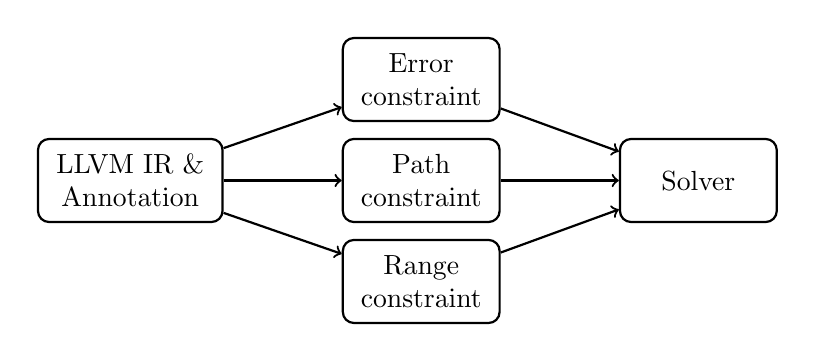
\begin{tikzpicture}[
	block/.style={
		rectangle, rounded corners,
		draw=black, thick,
		text width=5em, minimum height=3em, text centered
	},
	line/.style={draw, thick, ->},
	]
	\matrix[row sep=2mm, column sep=15mm] {
		& \node [block] (ec) {Error constraint}; & \\
		\node [block, text width=6em] (ir) {LLVM IR \& Annotation};
		& \node [block] (pc) {Path constraint};
		& \node [block] (sol) {Solver}; \\
		& \node [block] (rc) {Range constraint}; & \\
	};

	\path [line] (ir) -- (ec);
	\path [line] (ir) -- (pc);
	\path [line] (ir) -- (rc);
	\path [line] (ec) -- (sol);
	\path [line] (pc) -- (sol);
	\path [line] (rc) -- (sol);
\end{tikzpicture}

}
\caption{\sys's workflow.}
\label{f:flow}
\end{figure}

\subsection{Transformations}

In addition to standard optimizations like constant propagation,
\sys performs a series of code transformations to generate better
constraints for integer operations.  As discussed in \autoref{s:imply},
these transformations should not destroy the error preconditions
of integer operations.

\paragraph{Pointer arithmetic.}
In general \sys considers the result of a pointer arithmetic as a
black box, which can be any integral value within its range.

pointer subtraction is commonly used.

- symbolic~\cite{engelen:symbolic}.

\paragraph{Value equality testing.}
How to determine the values from two load instructions
are the same? Load hoisting, unsound aliasing rules.

\autoref{f:hoist} shows in the hoisting algorithm.

aliasing assumption~\cite{livshits:ipssa}.
\sys assumes that a pointer passed as a function parameter or a
global variable points is distinct from any other memory location.


\begin{figure}
\begin{algorithmic}
\footnotesize
\Procedure{Hoist}{$I$}\Comment{$I$ is a load instruction}
\State $\mathit{loc} \gets I$'s memory location to load from
\Loop
\If{\textbf{not} \Call{HoistInBlock}{$I$, $\mathit{loc}$}}
	\State \Return
\EndIf
\State $\mathit{blk} \gets$ \Call{ChooseTargetBlock}{$I$, $\mathit{loc}$}
\If{$\mathit{blk} = \textbf{nil}$}
	\State \Return
\EndIf
\State Move $I$ to the end of $blk$
\EndLoop
\EndProcedure
\\
\Function{HoistInBlock}{$I$, $\mathit{loc}$}
\Loop
\State $\mathit{prev} \gets I$'s previous instruction in current block
\If{$\mathit{prev} = \textbf{nil}$}
	\Comment{Moved to beginning of the block?}
	\State \Return \textbf{true}
\EndIf
\If{$\mathit{prev}$ may modify $\mathit{loc}$ \textbf{or} \\
\hspace{3.6em} \textbf{not} $\mathit{loc}$ dominates $\mathit{prev}$}
	\State \Return \textbf{false}
\EndIf
\State Move $I$ before $\mathit{prev}$
\EndLoop
\EndFunction
\\
\Function{ChooseTargetBlock}{$I$, $\mathit{loc}$}
\State $\mathit{blk} \gets I$'s block
\State $\mathit{anc} \gets$ the common ancestor of $\mathit{blk}$'s predecessor(s)
\If{$\mathit{anc} = \mathit{blk}$ \textbf{or} \textbf{not} $\mathit{loc}$ dominates $\mathit{anc}$}
	\State \Return \textbf{nil}
\EndIf
\State $\mathit{blkset} \gets \{\mathit{anc}\}$
\If{\Call{CanBlocksModify}{$\mathit{loc}$, $blk$, $\mathit{blkset}$}}
	\State \Return \textbf{nil}
\EndIf
\State \Return $\mathit{anc}$
\EndFunction
\\
\Function{CanBlocksModify}{$\mathit{loc}$, $\mathit{blk}$, $\mathit{blkset}$}
\ForAll{$b \in \mathit{blk}$'s predecessor(s)}
	\If{$b \notin \mathit{blkset}$}
		\State $\mathit{blkset} \gets \mathit{blkset} \cup \{b\}$
		\ForAll{$\mathit{instr} \in b$}
			\Comment{Can $b$ modify $\mathit{loc}$?}
			\If{$\mathit{instr}$ may modify $\mathit{loc}$}
				\State \Return \textbf{true}
			\EndIf
		\EndFor
		\If{\Call{CanBlocksModify}{$\mathit{loc}$, $b$, $\mathit{blkset}$}}
			\State \Return \textbf{true}
		\EndIf
	\EndIf
\EndFor
\State \Return \textbf{false}
\EndFunction

\end{algorithmic}

\caption{The hoisting algorithm to move a load instruction to the
earliest possible point within a function.  It repeats the two
phases: first try to move the instruction to the beginning of its
basic block; if successful, try to move it into the common ancestor
of the block's predecessors.}
\label{f:hoist}
\end{figure}

\paragraph{Error-before-check.}
An integer error check may come after the overflowed computation,
but before any use of the result.  In that case, the overflowed
computation is benign.  Below is such an example.  Even the
multiplication $x \times_u y$ overflows, the product \cc{size} is
not used before the check.
\begin{Verbatim}[commandchars=\\\{\},codes={\catcode`\$=3\catcode`\^=7\catcode`\_=8}]
\PY{k+kt}{unsigned} \PY{n}{size} \PY{o}{=} \PY{n}{x} \PY{o}{*} \PY{n}{y}\PY{p}{;}
\PY{k}{if} \PY{p}{(}\PY{n}{x} \PY{o}{\PYZgt{}} \PY{n}{UINT\PYZus{}MAX} \PY{o}{/} \PY{n}{y}\PY{p}{)}
    \PY{k}{return} \PY{o}{-}\PY{l+m+mi}{1}\PY{p}{;}
\PY{p}{.}\PY{p}{.}\PY{p}{.} \PY{o}{=} \PY{n}{malloc}\PY{p}{(}\PY{n}{size}\PY{p}{)}\PY{p}{;}
\end{Verbatim}


To avoid warning against such cases, \sys invokes LLVM to push every
integer operation down to the latest possible point along the control
flow, so that the result is computed only when it is needed.  The
detail of the algorithm is omitted since it is similar to load
hoisting, except that it runs towards the opposite direction, and
does not need to consider memory loads and stores.

In the above example, \sys will move the integer operation $x
\times_u y$ down to right after the \cc{if} branch and before the
\cc{malloc} call, where its result \cc{size} is first used.

\paragraph{Overflowed checking idiom.}
It is commonly seen in practice to use an overflowed result to do
the integer error check for $x +_u y$, where $x$ and $y$ are
of type \cc{unsigned int}, as follows.
\begin{align}
x +_u y <_u x.
\end{align}
This is equivalent to a ``sane'' check
$\cc{UINT_MAX} - x >_u y$.

Note that using overflowed result to check multiplication is trickier.
In general $x \times_u y <_u x$ is not a valid integer error check.
For example, given $\cc{maxnum} = \cc{0x1fffffff}$, $\cc{maxnum}
\times_u 16$ gives a larger value $\cc{0xfffffff0}$, which both
overflows and bypasses the check.  A correct check is $(x \times_u
y) /_u y \neq x$ or a sane form, $\cc{UINT_MAX} /_u x > y$.

Whether the imperfect check will lead to a security vulnerability
depends on the context.  In the example above, \cc{maxnum} has to
be at least $2^{28}$ to overflow $\cc{maxnum} \times 16$, and the
product must be greater than or equal to that to bypass the check
$\cc{maxnum} \times_u 16 <_u \cc{maxnum}$.  Allocating $2^{28}$
bytes (i.e., 256~MB) is possible in a userspace application, but
unlikely to succeed in the Linux kernel with \cc{kmalloc}, which
imposes a relatively small limit~\cite[\chapterautorefname~8]{ldd3}.
Nevertheless, the check becomes dangerous where the allocation
function used has a bigger limit (e.g., \cc{vmalloc}), the
multiplication is $\cc{maxnum} \times_u 1024$ (i.e., allocating
4~MB), or the \cc{kmalloc} limit is raised in the future.

\sys recognizes XXX integer error checking idioms...

\subsection{Error Constraint Generation}

\paragraph{Conversion constraint.}
\sys by default does not generate constraints for checking integer
conversions.  One may simply invoke GCC with \cc{-Wconversion} to
inspect potentially dangerous conversions.
[[[\sys does something for critical integers, array indices, annotated sizes.]]]

\paragraph{In-loop constraint.}
Move in-loop constraints out.

\subsection{Path Constraint Generation}

Path constraint generation.

unroll loops once.

handle comparison like \cc{p == NULL}.

\begin{figure}
\begin{algorithmic}
\Function{PathConstraint}{$\mathit{blk}$}
\State $g \gets \textbf{false}$
\ForAll{$\mathit{pred} \in \mathit{blk}$'s predecessors(s)}
\State $e \gets (\mathit{pred},\mathit{blk})$
\If{$e$ is not a back edge}
	\State $\mathit{br} \gets e$'s branching condition
	\State $\mathit{as} \gets \bigwedge_i(x_i = y_i)$ for all assignments along $e$
	\State $g \gets g \lor (\Call{PathConstraint}{\mathit{pred}} \land \mathit{br} \land \mathit{as})$
\EndIf
\EndFor
\State \Return{$g$}
\EndFunction
\end{algorithmic}

\caption{Algorithm for path constraint generation.}
\label{f:path-cstr}
\end{figure}

\subsection{Range Constraint Generation}

Range constraint \& annotations?

\subsection{Limitations}

miss bugs in some configurations, architectures,
and assembly code.
